\documentclass[fleqn]{article}
\usepackage[nodisplayskipstretch]{setspace}
\usepackage{amsmath, nccmath}
\usepackage{amssymb}
\usepackage{enumitem}
\usepackage{etoolbox}
\usepackage{graphicx}

\newcommand{\zerodisplayskip}{
	\setlength{\abovedisplayskip}{0pt}%
	\setlength{\belowdisplayskip}{0pt}%
	\setlength{\abovedisplayshortskip}{0pt}%
	\setlength{\belowdisplayshortskip}{0pt}%
	\setlength{\mathindent}{0pt}}

\makeatletter
	\newenvironment{equationCenter}{\@fleqnfalse\begin{equation*}}{\end{equation*}}
\makeatother

\title{Homework 4}
\author{Owen Sowatzke}
\date{October 16, 2023}

\begin{document}
	\offinterlineskip
	\setlength{\lineskip}{12pt}
	\zerodisplayskip
	\maketitle
	
	\begin{enumerate}[nolistsep]
		\item Define $T \in \mathcal{L}(\mathbb{F}^2)$ by
		
			\begin{equationCenter}
				T(w,z) = (z,w)
			\end{equationCenter}
			
			Find all eigenvalues and eigenvectors of $T$.
	
			$Tv = {\lambda}v$
			%
			$\Rightarrow T(w,z) = \lambda(w,z)$
			%
			$\Rightarrow(z,w) = \lambda(w,z)$
			%
			$\Rightarrow(z,w) = ({\lambda}w,{\lambda}z)$
			
			$z = {\lambda}w$
			%
			$\Rightarrow w = \lambda({\lambda}w)$
			%
			$\Rightarrow w = {\lambda}^2 w$
			%
			$\Rightarrow {\lambda}^2 = 1$
			%
			$\Rightarrow \lambda = \pm \sqrt{1}$
			%
			$\Rightarrow \lambda = \pm 1$
			
			$\therefore \lambda_1 = 1,\ \lambda_2 = -1$
			
			$\lambda_1 = 1 \Rightarrow z = w \Rightarrow v_1 = (w, w)$
			
			$\lambda_2 = -1 \Rightarrow z = -w \Rightarrow v_2 = (w, -w)$
			
		\item Suppose $T \in \mathcal{L}$ and $\text{dim range}\ T = k$. Prove that $T$ has at most $k + 1$ distinct eigenvalues.
	
			Let $v_j$ be an eigenvector of $T$. Then, $Tv_j = {\lambda_j}v_j$.
			
			Consider $\lambda_j \neq 0$:
			
			\begin{equation*}
				\Rightarrow \frac{1}{\lambda_j}T(v_j) = v_j \Rightarrow T\left(\frac{v_j}{\lambda_j}\right) = v_j	 \Rightarrow v_j \in \mathcal{R}(T)			
			\end{equation*}
			
			There are at most $k$ linearly independent eigenvectors $v_j$.
			
			For $\lambda_j$ to be distinct eigenvalues, each $v_j$ must be linearly independent.
			
			$\therefore$ there can be at most $k$ distinct nonzero eigenvalues $\lambda_j$.
			
			\pagebreak
			Consider $\lambda_j = 0$:
			
			For $\lambda_j=0$, there must be a nonzero eigenvector $v_j$ s.t.
			
			$Tv_j = 0 \Rightarrow v_j \in n(T)$
			
			Let $n(T) \neq \{0\} \Rightarrow \exists\ v_j \neq 0$ s.t. $Tv_j = 0$
			
			For this case, $\exists\ \lambda_j = 0$
			
			$\therefore$ there are at most $k + 1$ distinct eigenvalues.
		
		\item \textbf{Electrical Oscillators:} Consider the electric circuit shown below.
		
			{\centering
				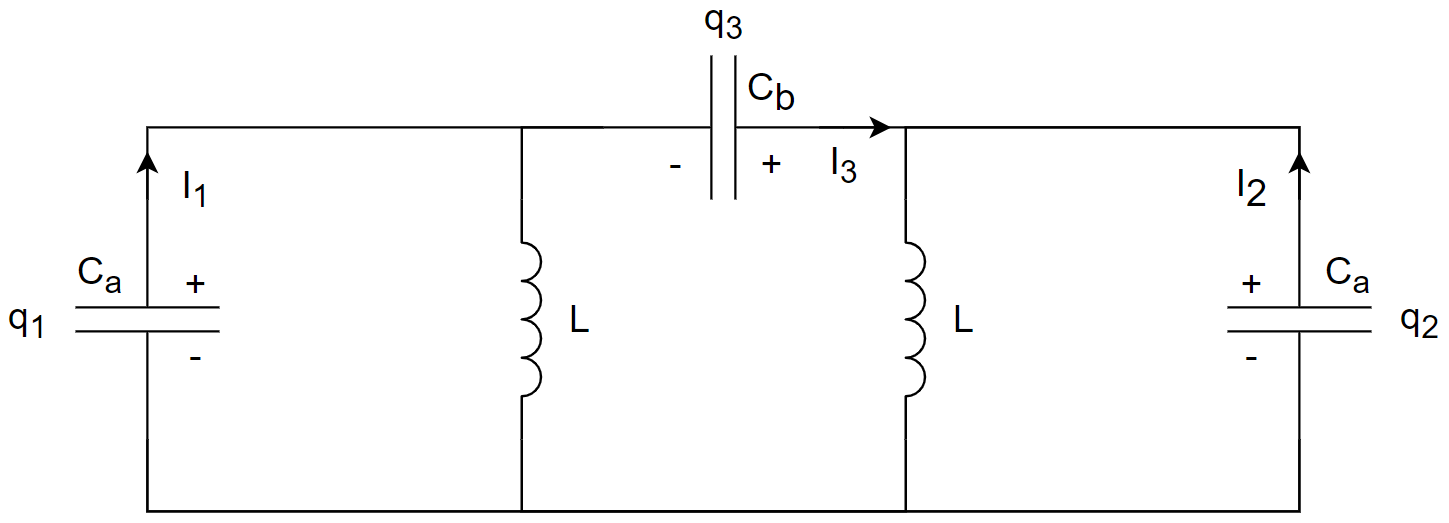
\includegraphics[width=0.75\textwidth]{Homework4_Circuit_Sowatzke.png}
			\par}
			
			Three capacitors (two with capacitance $C_a$ and one with capacitance $C_b$) are charged with (potentially different) charges $q_1$, $q_2$, and $q_3$ and connected with the polarity shown to two inductors of inductance $L$.
			
			In this problem we will explore how to convert the physical properties of this system into a linear map and how, with a strategic choice, we can convert the general linear map into an \textit{eigenvalue equation} that describes the system. In future homework problems, we will work on solving the \textit{eigenvalue equation} to determine the \textit{natural modes} of the system
			
			\begin{enumerate}[nolistsep]
				\item Remembering that the voltage difference across a capacitor and inductor can be written as $V=q/C$ and $V=L(dI/dt)$, respectively ($I$ is the \textit{net} current through the inductor), derive two equations that relate the charges $q_1$ and $q_2$ to the loop currents $I_1$, $I_2$, and $I_3$.
				
					\pagebreak
					\begin{equation*}
						\frac{q_1}{C_a} = L\frac{d}{dt}(I_1 - I_3)\Rightarrow q_1 = LC_a\frac{d}{dt}(I_1 - I_3)
					\end{equation*}
					%
					\begin{equation*}
						\frac{q_2}{C_a} = L\frac{d}{dt}(I_2 + I_3) \Rightarrow q_2 = LC_a\frac{d}{dt}(I_2 + I_3)
					\end{equation*}
				
				\item Remember that $I=dq/dt=\dot{q}$ and rewrite the equations so that they now relate $q_1$ and $q_2$ to $\ddot{q_1}$, $\ddot{q_2}$, and $\ddot{q_3}$.
				
					$q_1 = LC_a(\ddot{q_1} - \ddot{q_3})$
					
					$q_2 = LC_a(\ddot{q_2} + \ddot{q_3})$
					
				\item Using $V=q/C$, derive a relationship between $q_1$, $q_2$, and $q_3$. Take multiple time derivatives to convert this into a relationship between $\ddot{q_1}$, $\ddot{q_2}$, and $\ddot{q_3}$. Use this result to eliminate $\ddot{q_3}$ from your expressions for $q_1$ and $q_2$.
				
					\begin{equation*}
						\frac{q_1}{C_a} + \frac{q_3}{C_b} = \frac{q_2}{C_a} \Rightarrow \frac{\ddot{q_1}}{C_a} + \frac{\ddot{q_3}}{C_b} = \frac{\ddot{q_2}}{C_a}
					\end{equation*}
					%
					\begin{equation*}
						 \Rightarrow \frac{\ddot{q_3}}{C_b} = \frac{\ddot{q_2}}{C_a} - \frac{\ddot{q_1}}{C_a} \Rightarrow \ddot{q_3} = \frac{C_b}{C_a}(\ddot{q_2} - \ddot{q_1})
					\end{equation*}
					%
					\begin{equation*}
						q_1 = LC_a\left(\ddot{q_1} - \frac{C_b}{C_a}(\ddot{q_2} - \ddot{q_1})\right) \Rightarrow q_1 = LC_a\ddot{q_1} - LC_b(\ddot{q_2} - \ddot{q_1})
					\end{equation*}
					%
					$\Rightarrow q_1 = LC_a\ddot{q_1} - LC_b\ddot{q_2} + LC_b\ddot{q_1} \Rightarrow q_1 = L(C_a + C_b)\ddot{q_1} - LC_b\ddot{q_2}$
					
					\begin{equation*}
						q_2 = LC_a\left(\ddot{q_2} + \frac{C_b}{C_a}(\ddot{q_2} - \ddot{q_1})\right) \Rightarrow q_2 = LC_a\ddot{q_2} + LC_b(\ddot{q_2} - \ddot{q_1})
					\end{equation*}
					%
					$\Rightarrow q_2 = LC_a\ddot{q_2} + LC_b\ddot{q_2} - LC_b\ddot{q_1} \Rightarrow q_2 = - LC_b\ddot{q_1} + L(C_a + C_b)\ddot{q_2}$
					
				\item Algebraically rearrange these equations into the following matrix form:
				
					\begin{equationCenter}
						\begin{bmatrix}\ddot{q_1} \\ \ddot{q_2}\end{bmatrix} = M \begin{bmatrix}q_1 \\ q_2\end{bmatrix}
					\end{equationCenter}
					
					where $M$ is a $2 \times 2$ matrix.
					
					\pagebreak
					\begin{equation*}
						q_1 = L(C_a + C_b)\ddot{q_1} - LC_b\ddot{q_2} \Rightarrow LC_b\ddot{q_2} = L(C_a + C_b)\ddot{q_1} - q_1
					\end{equation*}
					%
					\begin{equation*}
						\Rightarrow \ddot{q_2} = \frac{C_a + C_b}{C_b}\ddot{q_1} - \frac{1}{LC_b}q_1
					\end{equation*}
					%
					\begin{equation*}
						q_2 = - LC_b\ddot{q_1} + L(C_a + C_b)\ddot{q_2}
					\end{equation*}
					%
					\begin{equation*}
						\Rightarrow q_2 = - LC_b\ddot{q_1} + L(C_a + C_b)\left(\frac{C_a + C_b}{C_b}\ddot{q_1} - \frac{1}{LC_b}q_1\right)
					\end{equation*}
					%
					\begin{equation*}
						\Rightarrow q_2 = - LC_b\ddot{q_1} + \frac{L(C_a + C_b)^2}{C_b}\ddot{q_1} - \frac{C_a + C_b}{C_b}q_1
					\end{equation*}
					%
					\begin{equation*}
						\Rightarrow q_2 = - LC_b\ddot{q_1} + \frac{L(C_a^2 + 2C_aC_b + C_b^2)}{C_b}\ddot{q_1} - \frac{C_a + C_b}{C_b}q_1
					\end{equation*}
					%
					\begin{equation*}
						\Rightarrow q_2 = \frac{L(C_a^2 + 2C_aC_b + C_b^2) - LC_b^2}{C_b}\ddot{q_1} - \frac{C_a + C_b}{C_b}q_1
					\end{equation*}
					%
					\begin{equation*}
						\Rightarrow q_2 = \frac{L(C_a^2 + 2C_aC_b)}{C_b}\ddot{q_1} - \frac{C_a + C_b}{C_b}q_1
					\end{equation*}
					%
					\begin{equation*}
						\Rightarrow q_2 = \frac{LC_a(C_a + 2C_b)}{C_b}\ddot{q_1} - \frac{C_a + C_b}{C_b}q_1
					\end{equation*}
					%
					\begin{equation*}
						\Rightarrow \frac{LC_a(C_a + 2C_b)}{C_b}\ddot{q_1} = \frac{C_a + C_b}{C_b}q_1 + q_2
					\end{equation*}
					%
					\begin{equation*}
						\Rightarrow \ddot{q_1} = \frac{C_a + C_b}{LC_a(C_a + 2C_b)}q_1 + \frac{C_b}{LC_a(C_a + 2C_b)}q_2
					\end{equation*}
					%
					\begin{equation*}
						\ddot{q_2} = \frac{C_a + C_b}{C_b}\ddot{q_1} - \frac{1}{LC_b}q_1
					\end{equation*}
					%
					\begin{equation*}
						\Rightarrow \ddot{q_2} = \frac{C_a + C_b}{C_b}\left(\frac{C_a + C_b}{LC_a(C_a + 2C_b)}q_1 + \frac{C_b}{LC_a(C_a + 2C_b)}q_2\right) - \frac{1}{LC_b}q_1
					\end{equation*}
					%
					\begin{equation*}
						\Rightarrow \ddot{q_2} = \frac{(C_a + C_b)^2}{LC_aC_b(C_a + 2C_b)}q_1 + \frac{C_a + C_b}{LC_a(C_a + 2C_b)}q_2 - \frac{1}{LC_b}q_1
					\end{equation*}
					%
					\begin{equation*}
						\Rightarrow \ddot{q_2} = \frac{(C_a + C_b)^2 - C_a(C_a + 2C_b)}{LC_aC_b(C_a + 2C_b)}q_1 + \frac{C_a + C_b}{LC_a(C_a + 2C_b)}q_2
					\end{equation*}
					%
					\begin{equation*}
						\Rightarrow \ddot{q_2} = \frac{C_a^2 + 2C_aC_b + C_b^2 - C_a^2 - 2C_aC_b}{LC_aC_b(C_a + 2C_b)}q_1 + \frac{C_a + C_b}{LC_a(C_a + 2C_b)}q_2
					\end{equation*}
					%
					\begin{equation*}
						\Rightarrow \ddot{q_2} = \frac{C_b^2}{LC_aC_b(C_a + 2C_b)}q_1 + \frac{C_a + C_b}{LC_a(C_a + 2C_b)}q_2
					\end{equation*}
					%
					\begin{equation*}
						\Rightarrow \ddot{q_2} = \frac{C_b}{LC_a(C_a + 2C_b)}q_1 + \frac{C_a + C_b}{LC_a(C_a + 2C_b)}q_2
					\end{equation*}
			\end{enumerate}
	\end{enumerate}
\end{document}